
\chapter{Some parameterized functions} \label{appB}

\graphicspath{{AppendixB_ys/}}


In the parametrization method developed in chapter \ref{ch:Parametrization}, one fundamental problem is to choose the function to fit each components of the frequency spectra. First, the function should be able to be characterized by a limited number of parameters. Then, considering the frequency spectra to be fitted, the functions should be continuous and supported on the whole range of real number. In order to represent the most basic features of one spectra, at least three parameters (amplitude, position and shape) are required. Although the asymmetry could occur in the real spectra, in this study, we assume that the spectra are symmetrical with respect to the central position. An asymmetry of spectra can be introduced in the future work.  


\section*{The Gaussian function}


The Gaussian (normal) function is the most common continuous distribution function that has been extensively used in the spectrum fitting for many application. The expression of the Gaussian function is:%
%%%%%%%%%%%%%%%%%%%%
\begin{equation}
f(x) = A\exp\biggl[-\frac{1}{2}\left(\frac{x-\mu}{\sigma}\right)^2\biggr],
\label{eq:GD}
\end{equation}
%%%%%%%%%%%%%%%%%%%%
\noindent where $A$ (the amplitude), $\mu$ (the mean or expectation of the distribution) and $\sigma$ (the standard deviation) represent the intensity, central position and shape of the distribution (spectrum). The Gaussian function has been used to fit both the direct current (DC) and low-frequency (LF) components of spectra in this study. Then, the parameters (e.g., $\sigma_\mathrm{LF}$ for the LF width) could be obtained directly from the fitting results. 


\section*{The Generalized Gaussian function}



Instead of using a fixed exponent (2) as GD, the generalized Gaussian (GG) function has one more parameter to represent a varying exponent:%
%%%%%%%%%%%%%%%%%%%%
\begin{equation}
G(x) = A\exp\biggl[-\left(\frac{|f-\mu|}{\alpha}\right)^{\beta}\biggr],
\label{eq:GGD}
\end{equation}
%%%%%%%%%%%%%%%%%%%%
\noindent here, the parameter $\beta$ is the added parameter to give more flexibility of the shapes of the distributions. The standard deviation can be calculated by: $\alpha\sqrt{\frac{\Gamma(3/\beta)}{\Gamma(1/\beta)}}$, where $\Gamma()$ is the Gamma function. Since the standard deviation depends on two parameters, which make it difficult to control the parameter constraints in the fitting process, we introduce a modified GG function:%
%%%%%%%%%%%%%%%%%%%%
\begin{equation}
GG(x) = A\exp\biggl[-\left(\frac{|f-\mu|}{\sigma\sqrt(\gamma(1/\beta)/\gamma(3/\beta))}\right)^{\beta}\biggr],
\label{eq:GGD}
\end{equation}
%%%%%%%%%%%%%%%%%%%%
\noindent then, the standard deviation simply becomes $\sigma$. By varying the exponent parameter $\beta$, the GG function could smoothly change between different distribution (spectral) shapes. Specifically, the GG function reduces to the Gaussian function when $\beta = 2$, and $\beta = 1$ represents the Laplacian distribution. The frequently used Lorentzian (Cauchy) distribution corresponds to some $\beta$ value between 1 and 2. The GG function has high flexibility and clear meaning of each parameter. Figure \ref{fig:GGD_plot} shows some typical distribution shapes of the GG function with different $\beta$ ($\sigma = 50$). With the increase of $\beta$, the distribution changes from peaked shape with long tail to almost rectangle shape.  


%%%%%%%%%%%%%%%%%%%%
\begin{figure}[h]
\begin{centering}
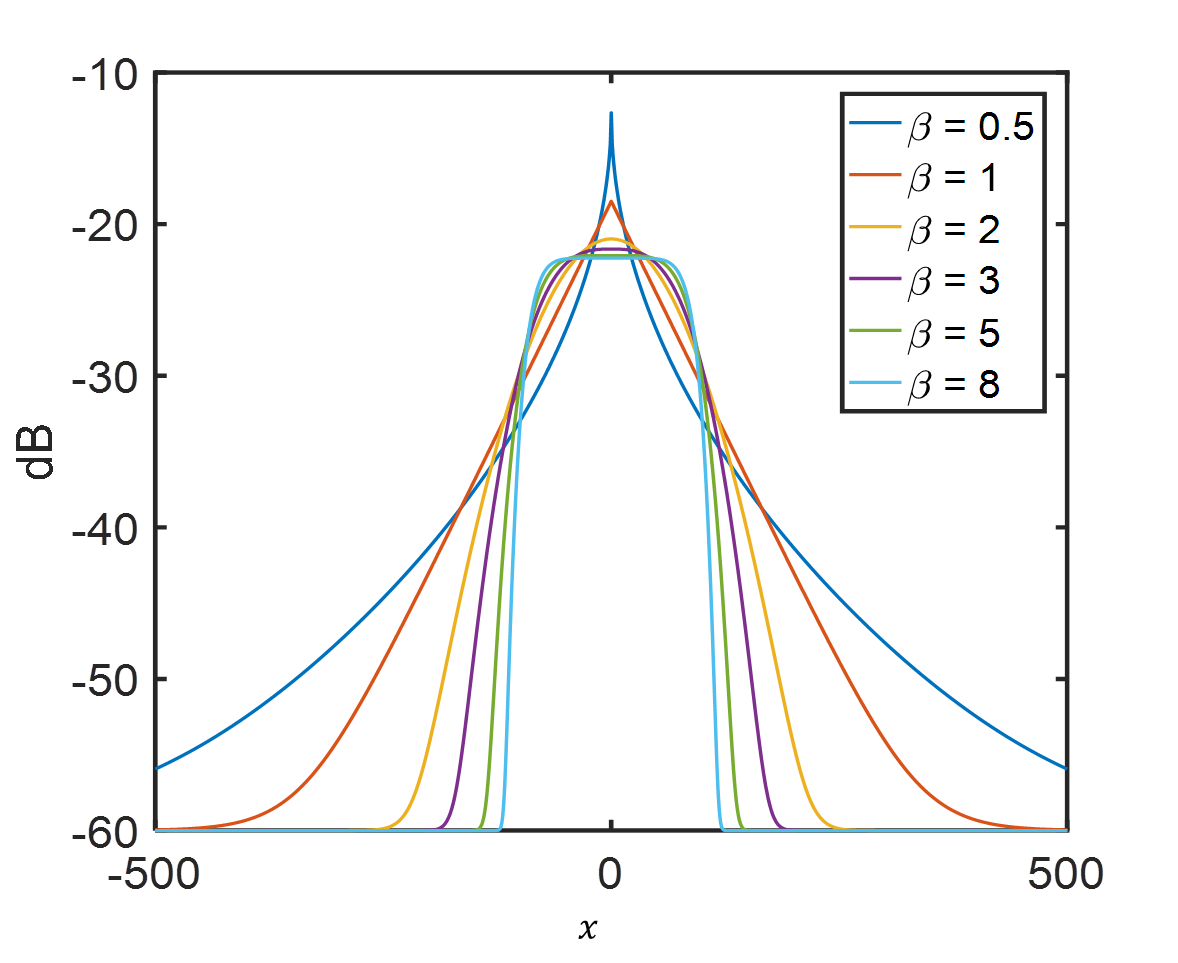
\includegraphics[scale=0.35]{fig_GGD_plot.png}
\par\end{centering}
\caption{Examples of some distributions of the GG function when changing the exponent parameter $\beta$.}
\label{fig:GGD_plot}
\end{figure}
%%%%%%%%%%%%%%%%%%%%


\section*{The Voigt function}


The Voigt function is a convolution of a Gaussian function and a Lorentzian function, which has been widely used in analyzing spectra data from spectroscopy and diffraction.
%%%%%%%%%%%%%%%%%%%%
\begin{equation}
V(x)= \int_{-\infty}^{\infty} G(x')L(x-x') dx'
\label{eq:VD}
\end{equation}
%%%%%%%%%%%%%%%%%%%%,
\noindent where $G(x) = \frac{1}{\sigma\sqrt{2\pi}}e^{-(x-\mu)^2/(2\sigma^2)}$ is the Gaussian function and $L(x) = \frac{\gamma}{\pi(x^2+\gamma^2)}$ the centered Lorentzian function. Note that the position parameter $\mu$ could be introduced in the Lorentzian function and accordingly the centered Gaussian function should be applied, which is equivalent. However, in calculating the convolution, the calculation of the Faddeeva function is very complicated and thus time consuming. Therefore, in practical application, an approximate function, called the pseudo-Voigt function is always used:%
%%%%%%%%%%%%%%%%%%%%
\begin{equation}
V_{p}(x) = \eta \cdot L(x) + (1-\eta) \cdot G(x),\quad 0\leq\eta\leq1.
\label{eq:VD}
\end{equation}
%%%%%%%%%%%%%%%%%%%%
\noindent Here, $\eta$ is the weight coefficient between the two functions. The pseudo-Voigt function is in fact a linear combination of the Gaussian and Lorentzian function. So its shape could still be limited by the two functions. 



\section*{The Taylor function}


The Taylor function is expressed as a fast Fourier transform (FFT) of a correlation correlation. When the correlation function is defined as:% 
%%%%%%%%%%%%%%%%%%%%
\begin{equation}
  F_{corr}(x) = \exp\left[-k^2u^2\tau^2\left(\frac{x}{\tau}-1+e^{-x/\tau}\right)\right],
  \label{eq:Fcorr}
\end{equation}
%%%%%%%%%%%%%%%%%%%%
\noindent defining $\Delta = k^2D = k^2u^2\tau$, where $D = u^2\tau$, the above expression becomes:%
%%%%%%%%%%%%%%%%%%%%
\begin{equation}
  F_{corr}(x) = \exp\left[-\Delta(x-\tau+e^{-t/\tau})\right],
  \label{eq:Fcorr}
\end{equation}
%%%%%%%%%%%%%%%%%%%%
\noindent then the Taylor is defined as the FFT of $F_{corr}$ and thus following the form:%
%%%%%%%%%%%%%%%%%%%%
\begin{equation}\label{eq:BBT}
  T(x) = \mathrm{FFT}\left\{\exp\left[-\Delta_{BB}(t-\tau_{BB}+e^{-t/\tau_{BB}})\right]\times\delta\varphi\right\},
\end{equation}
%%%%%%%%%%%%%%%%%%%%
\noindent with introducing the position parameter by adding $\delta\varphi = \exp(i2\pi\mu t)$. The high flexibility of the Taylor function is shown in figure \ref{fig:TD_plot}. Specifically, when $\Delta$ is relatively large ($\Delta = 1$), the distribution shape could change from Gaussian to Laplacian, and with smaller $\Delta$ ($\Delta = 0.1$), the Taylor function could cover the shapes similar with the Lorentzian distribution with long tails. 


%%%%%%%%%%%%%%%%%%%%
\begin{figure}[h]
\begin{centering}
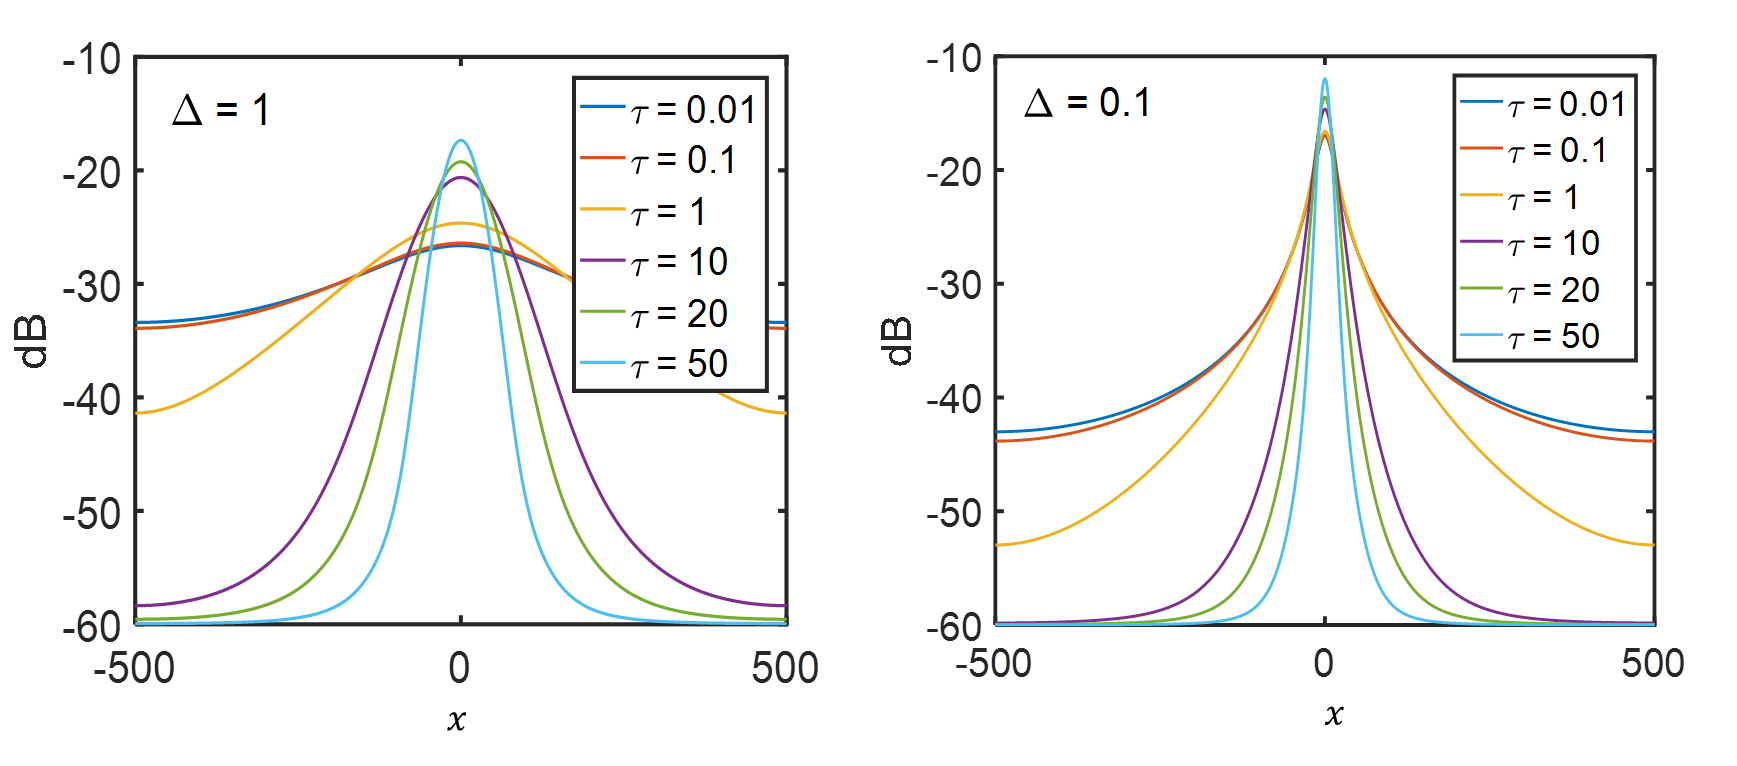
\includegraphics[scale=0.5]{fig_TD_plot.png}
\par\end{centering}
\caption{Examples of some distributions of the Taylor function when changing $\tau$ at two different $\Delta$.}
\label{fig:TD_plot}
\end{figure}
%%%%%%%%%%%%%%%%%%%%



%A third alternative model for the BB component is the Taylor function. It was used in \cite{Hennequin_1999_EPS,Casati_2009_thesis} to express the correlation function of a turbulence signal in plasma physics:%
%%%%%%%%%%%%%%%%%%%%%
%\begin{equation}\label{eq:Fcorr}
%  F_{corr}(k,u,\tau_{BB}) = \exp\left[-k^2u^2\tau_{BB}^2\left(\frac{t}{\tau_{BB}}-1+e^{-t/\tau_{BB}}\right)\right].
%\end{equation}
%%%%%%%%%%%%%%%%%%%%%
%\noindent Here, $k$, $u$ and $\tau_{BB}$ represent the wavenumber, velocity and correlation time of the turbulence, respectively, while $t$ is the sampling sequence, based on the theory of collective wave scattering by a non-uniform plasma \cite{Gresillon_1992_PPCF}. Since the velocity correlation $C_{v}=e^{-t/\tau_{BB}}$ was used, the correlation function above is referred to as the Taylor function. The corresponding frequency spectrum is calculated through the Fourier transform of $F_{corr}$.
%
%In scattering theory, long correlation lengths correspond to a convective Gaussian spectrum, while short correlation lengths have a diffusive Lorentzian spectrum. Accordingly, in $F_{corr}$, $ku\tau\gg1$ and $ku\tau\leq1$ lead to the convective and diffusive limit, respectively. Defining $\Delta=k^2D=k^2u^2\tau$, where $D=u^2\tau$ is the diffusion coefficient, and introducing the averaged shift parameter $\delta\varphi=\exp(i2\pi\mu_{BB}t)$, the Taylor model of the BB turbulence thus has the following form:%
%\begin{equation}\label{eq:BBT}
%  C_{BB}^{\textbf{Taylor}}=A_{BB} \times\mathrm{FFT}\left\{\exp\left[-\Delta_{BB}(t-\tau_{BB}+e^{-t/\tau_{BB}})\right]\times\delta\varphi\right\}.
%\end{equation}
%
%\noindent The connection to the transport coefficients can then be established by analysis of the fitting parameters.